\documentclass[10pt]{beamer}
\usetheme{Pittsburgh}
\setbeamertemplate{navigation symbols}{}
\setbeamertemplate{bibliography item}{\insertbiblabel}

\usepackage{graphicx}
\usepackage[linesnumbered,ruled,vlined]{algorithm2e}
\usepackage{color,soul}
\usepackage[utf8]{inputenc}
\usepackage[T1]{fontenc}
\usepackage{textcomp}
\usepackage{amsmath, amssymb}
\usepackage{caption}
\usepackage{listings}
\usepackage[italian]{babel}

% figure support
\usepackage{tikz}
\usetikzlibrary{calc}
\usepackage{import}
\usepackage{xifthen}
\usepackage{pdfpages}
\usepackage{transparent}
\usepackage[]{hyperref}
\usepackage{multirow}

% provides the H option
\usepackage{float}

% provides subcaptions
\usepackage{subcaption}

% provides justification
\usepackage{ragged2e}
\justifying

% for logo
\usepackage[export]{adjustbox}

\pdfsuppresswarningpagegroup=1
\setcounter{tocdepth}{1}
\AtBeginSection[]
{
  \begin{frame}<beamer>
    \tableofcontents[currentsection]
  \end{frame}
}

\logo{
\includegraphics[width=0.2\textwidth]{./img/logo_unipa.png}}
\author{Augello Andrea \and Castiglione Francesco Paolo \and La Martina Marco}
\institute{Università degli studi di Palermo}
\begin{document}
\title[Chang'e]{Documentazione - Progetto di Robotica}
	\begin{frame}
		\titlepage
	\end{frame}


	\section{Introduzione}\label{sec:Introduzione}
	\frame{\sectionpage}
	\frame{
		La pandemia del coronavirus SARS-CoV-2 ha dato una forte
		spinta alla ricerca sia nel campo sanitario che informatico, mettendo in
		evidenza forti carenze dal punto di vista infrastrutturale.
		
		
		Al momento, considerando la limitata disponibilità del vaccino alle masse, uno dei miglior modi di evitare la contrazione del coronavirus è
		di evitarne l'esposizione. Il distanziamento sociale si configura di
		conseguenza come un prerequisito per una significativa riduzione del numero
		di infetti, come evidenziato da simulazioni di un sistema ad agenti
		\cite{silva2020covid}. Un problema chiave risulta essere
		il controllo del rispetto delle norme di distanziamento all'interno degli
		spazi chiusi. 
	}

	\begin{frame}{Obbiettivo}
	L'obbiettivo del progetto è quello di sviluppare un robot con lo scopo di \textbf{evitare assembramenti in ambienti indoor} e di invitare a \textbf{rispettare le norme sul distanziamento sociale}. 
	
	Nella dimostrazione presentata il nostro robot rileva le persone nella stanza e individua i possibili assembramenti. In seguito alla fase di rilevazione si sposterà verso l'assembramento evitando gli ostacoli e, arrivato, esorterà le persone al rispetto del distanziamento sociale.
	\end{frame}
	
	\begin{frame}[allowframebreaks]{Stato dell'arte}
	Un TurtleBot 2, con una camera RGB-D e CCTV per il rilevamento degli assembramenti, una camera termica FLIR C3 per rilevare la temperatura corporea e un lidar 2-D per evitare le collisioni. L'elaborazione delle immagini provenienti da CCTV è eseguita in un laptop con una CPU Intel i7 7th generation e una GPU Nvidia GTX1060, mentre il resto dell'elaborazione è eseguita su una CPU Intel i9 8th generation e una GPU Nvidia RTX2080 montate sul robot.
	
	\begin{figure}[H]
		\centering
		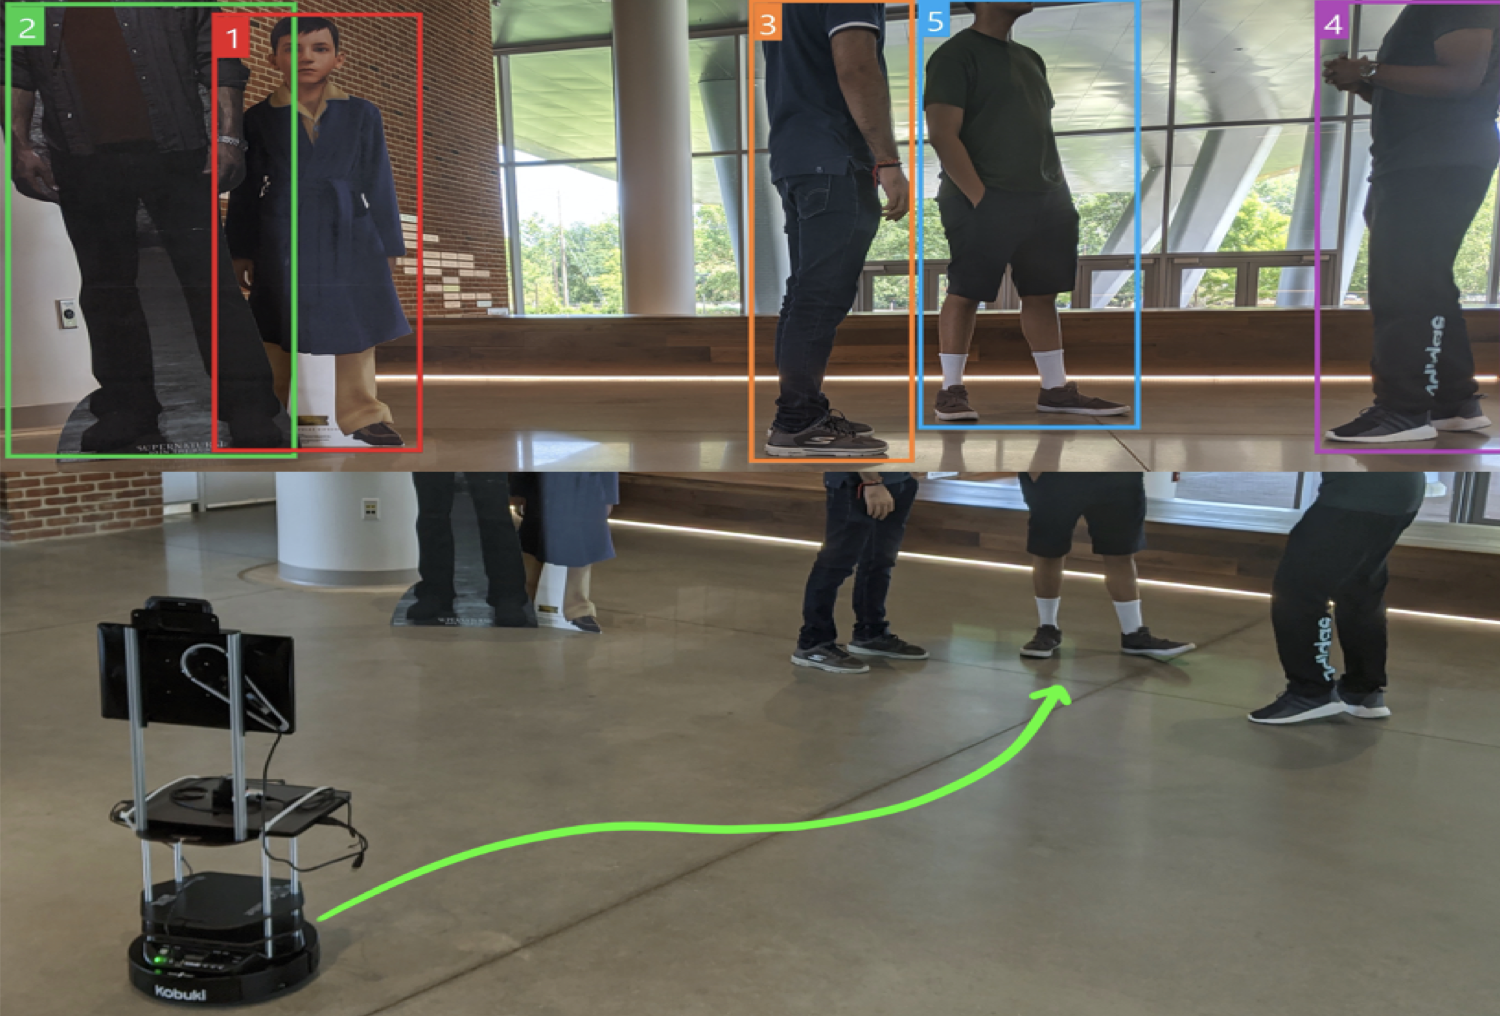
\includegraphics[width=0.6\linewidth]{./img/State_of_art_1.png}
	\end{figure}
	
	\framebreak
	
	Un Laikago con 2 camere laterali e CCTV per il rilevamento degli
		assembramenti e un lidar 3-D per evitare le collisioni. 
		L'elaborazione riguardante il modulo visivo è effettuata in una NVIDIA Jetson AGX Xavier,
		il resto è eseguito in una CPU Intel i5 8259U. Il rilevamento delle persone viene effettuato tramite la rete YOLO.
	
	\begin{figure}[H]
		\centering
		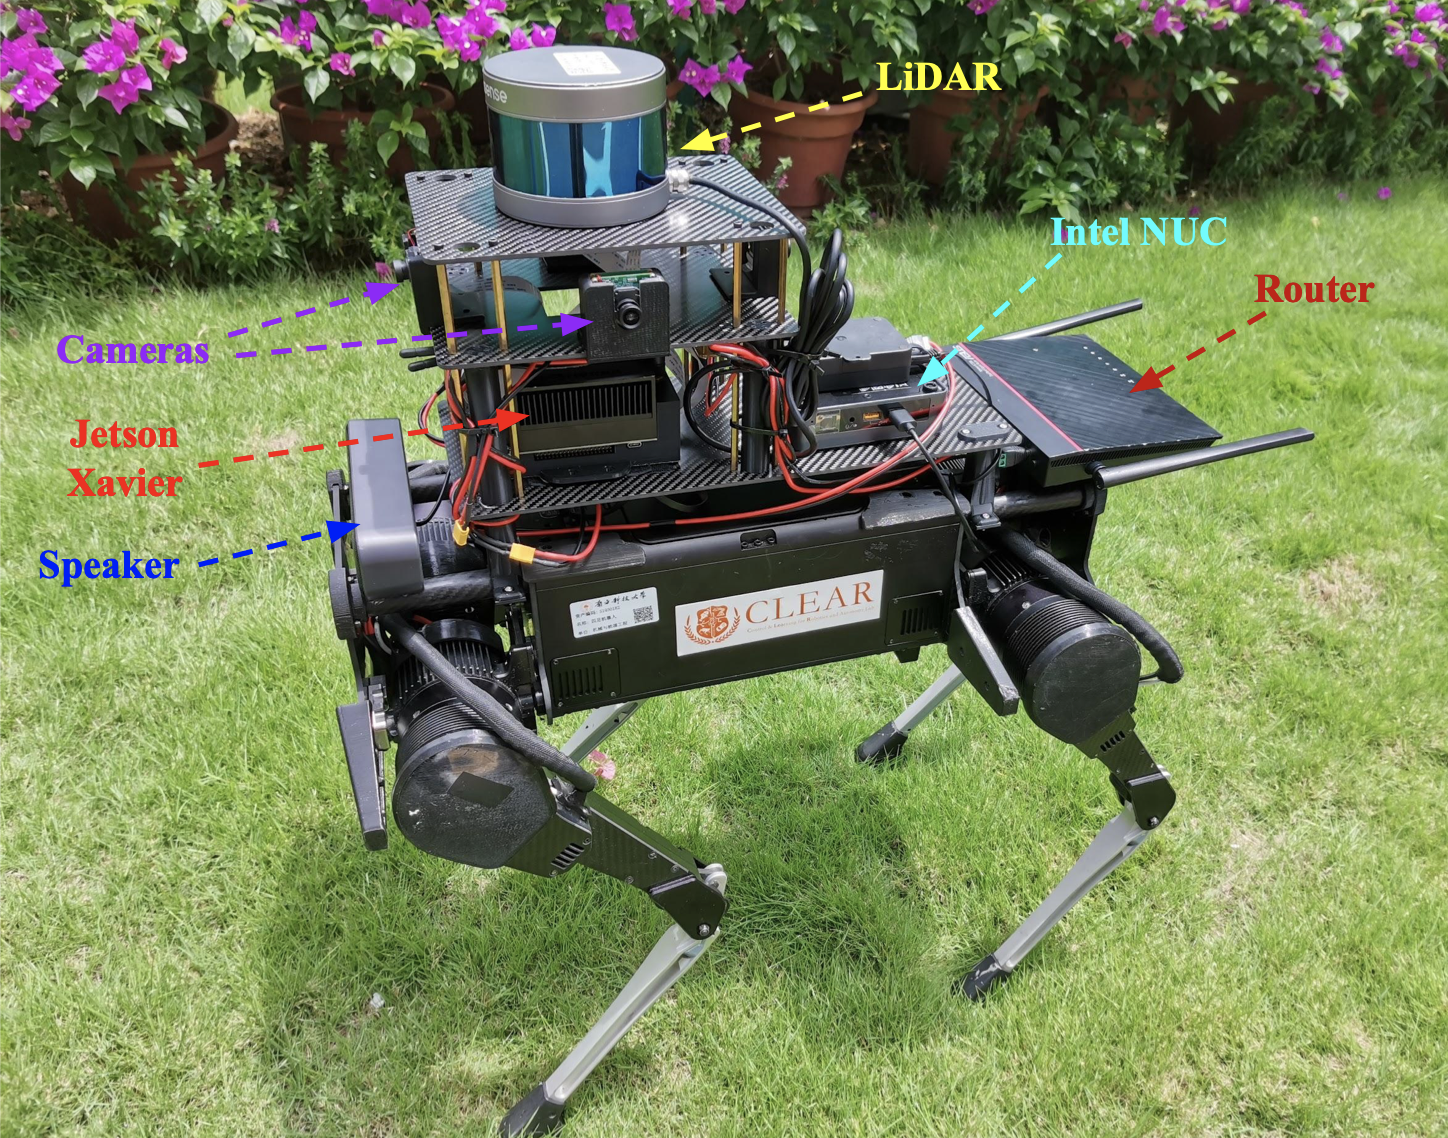
\includegraphics[width=0.6\linewidth]{./img/State_of_art_2.png}
	\end{figure}
	
	\end{frame}
	
	\begin{frame}{Setup}
	\centering
	\begin{tabular}{l l}
		\hline
		\textbf{OS} & Ubuntu 18.04 \\
					& Ubuntu 20.04 \\ 
					& Raspberry Pi OS Buster\\
		\textbf{ROS version} & melodic \\
							 & noetic \\ 
		\textbf{Webots}	& R2020b revision 1\\ 
		\textbf{OpenCV}~\cite{opencv} 	& 4.x \\
		\textbf{Imutils}~\cite{imutils} & 0.5.3 \\
		\textbf{Matplotlib}~\cite{matplotlib} & 3.3.3 \\
		\textbf{Numpy}~\cite{numpy} & 1.17.2 \\
		\textbf{Scikit-learn}~\cite{scikit} & 0.21.3\\
		\textbf{Raspberry} & Raspberry Pi 3B+ \\\hline
	\end{tabular}
	\end{frame}

	\section{TIAGo Iron}\label{sec:TIAGo-Iron} 
	\frame{\sectionpage}
	\frame{

	\begin{columns}
		\begin{column}{0.7\textwidth}
		\justifying
		Il robot scelto per l'obbiettivo proposto è il \textbf{TIAGo Iron}, un
		robot umanoide a due ruote con torso e testa ma senza braccia
		articolate \cite{pages2016tiago}.
		
		Il datasheet del \textbf{TIAGo} \cite{tiago_datasheet} indica la
		presenza di speaker e display, non  presenti nel modello Webots
		\cite{tiagoiron}, che sono quindi stati aggiunti.
		
		La camera del \textbf{TIAGo} è RGB-D ma il modello Webots ne è
		sprovvisto, di conseguenza è stata utilizzata una camera monoscopica
		RGB. 
		
		L'IMU utilizzata ha 6 gradi di libertà. 
		
		Il modello Webots del \textbf{TIAGo} presenta un lidar (Hokuyo
		URG-04LX-UG01 \cite{lidarspecs}) che, conformemente al datasheet,  ha
		un range di $5.6\,m$ ed un FOV di $240^{\circ}$ (agli estremi è
		parzialmente occluso).
		\end{column}
		
		\begin{column}{0.3\textwidth}
			\begin{figure}[htpb]
				\centering
				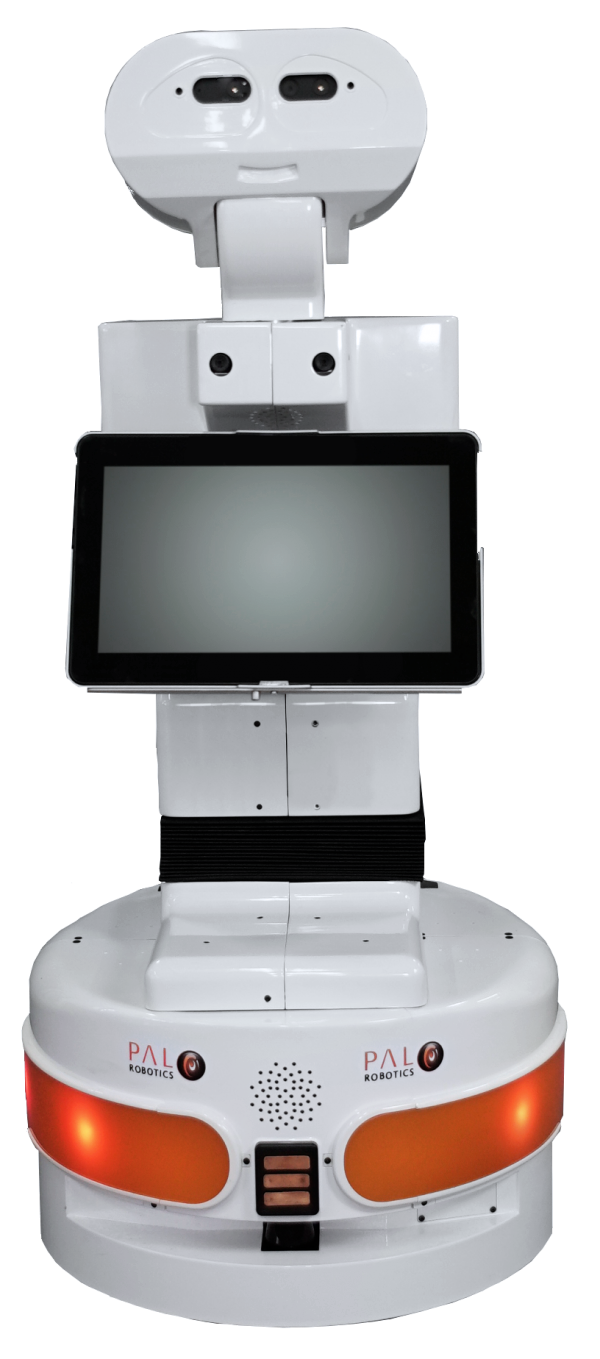
\includegraphics[width=\textwidth]{./img/tiago.png}
				\label{fig:tiago}
			\end{figure}
		\end{column}
	\end{columns}
	
	}

	\section{Gestione dei nodi ROS}\label{sec:Ros}
	\frame{\sectionpage}

	\frame{\begin{figure}[H]
		\centering
		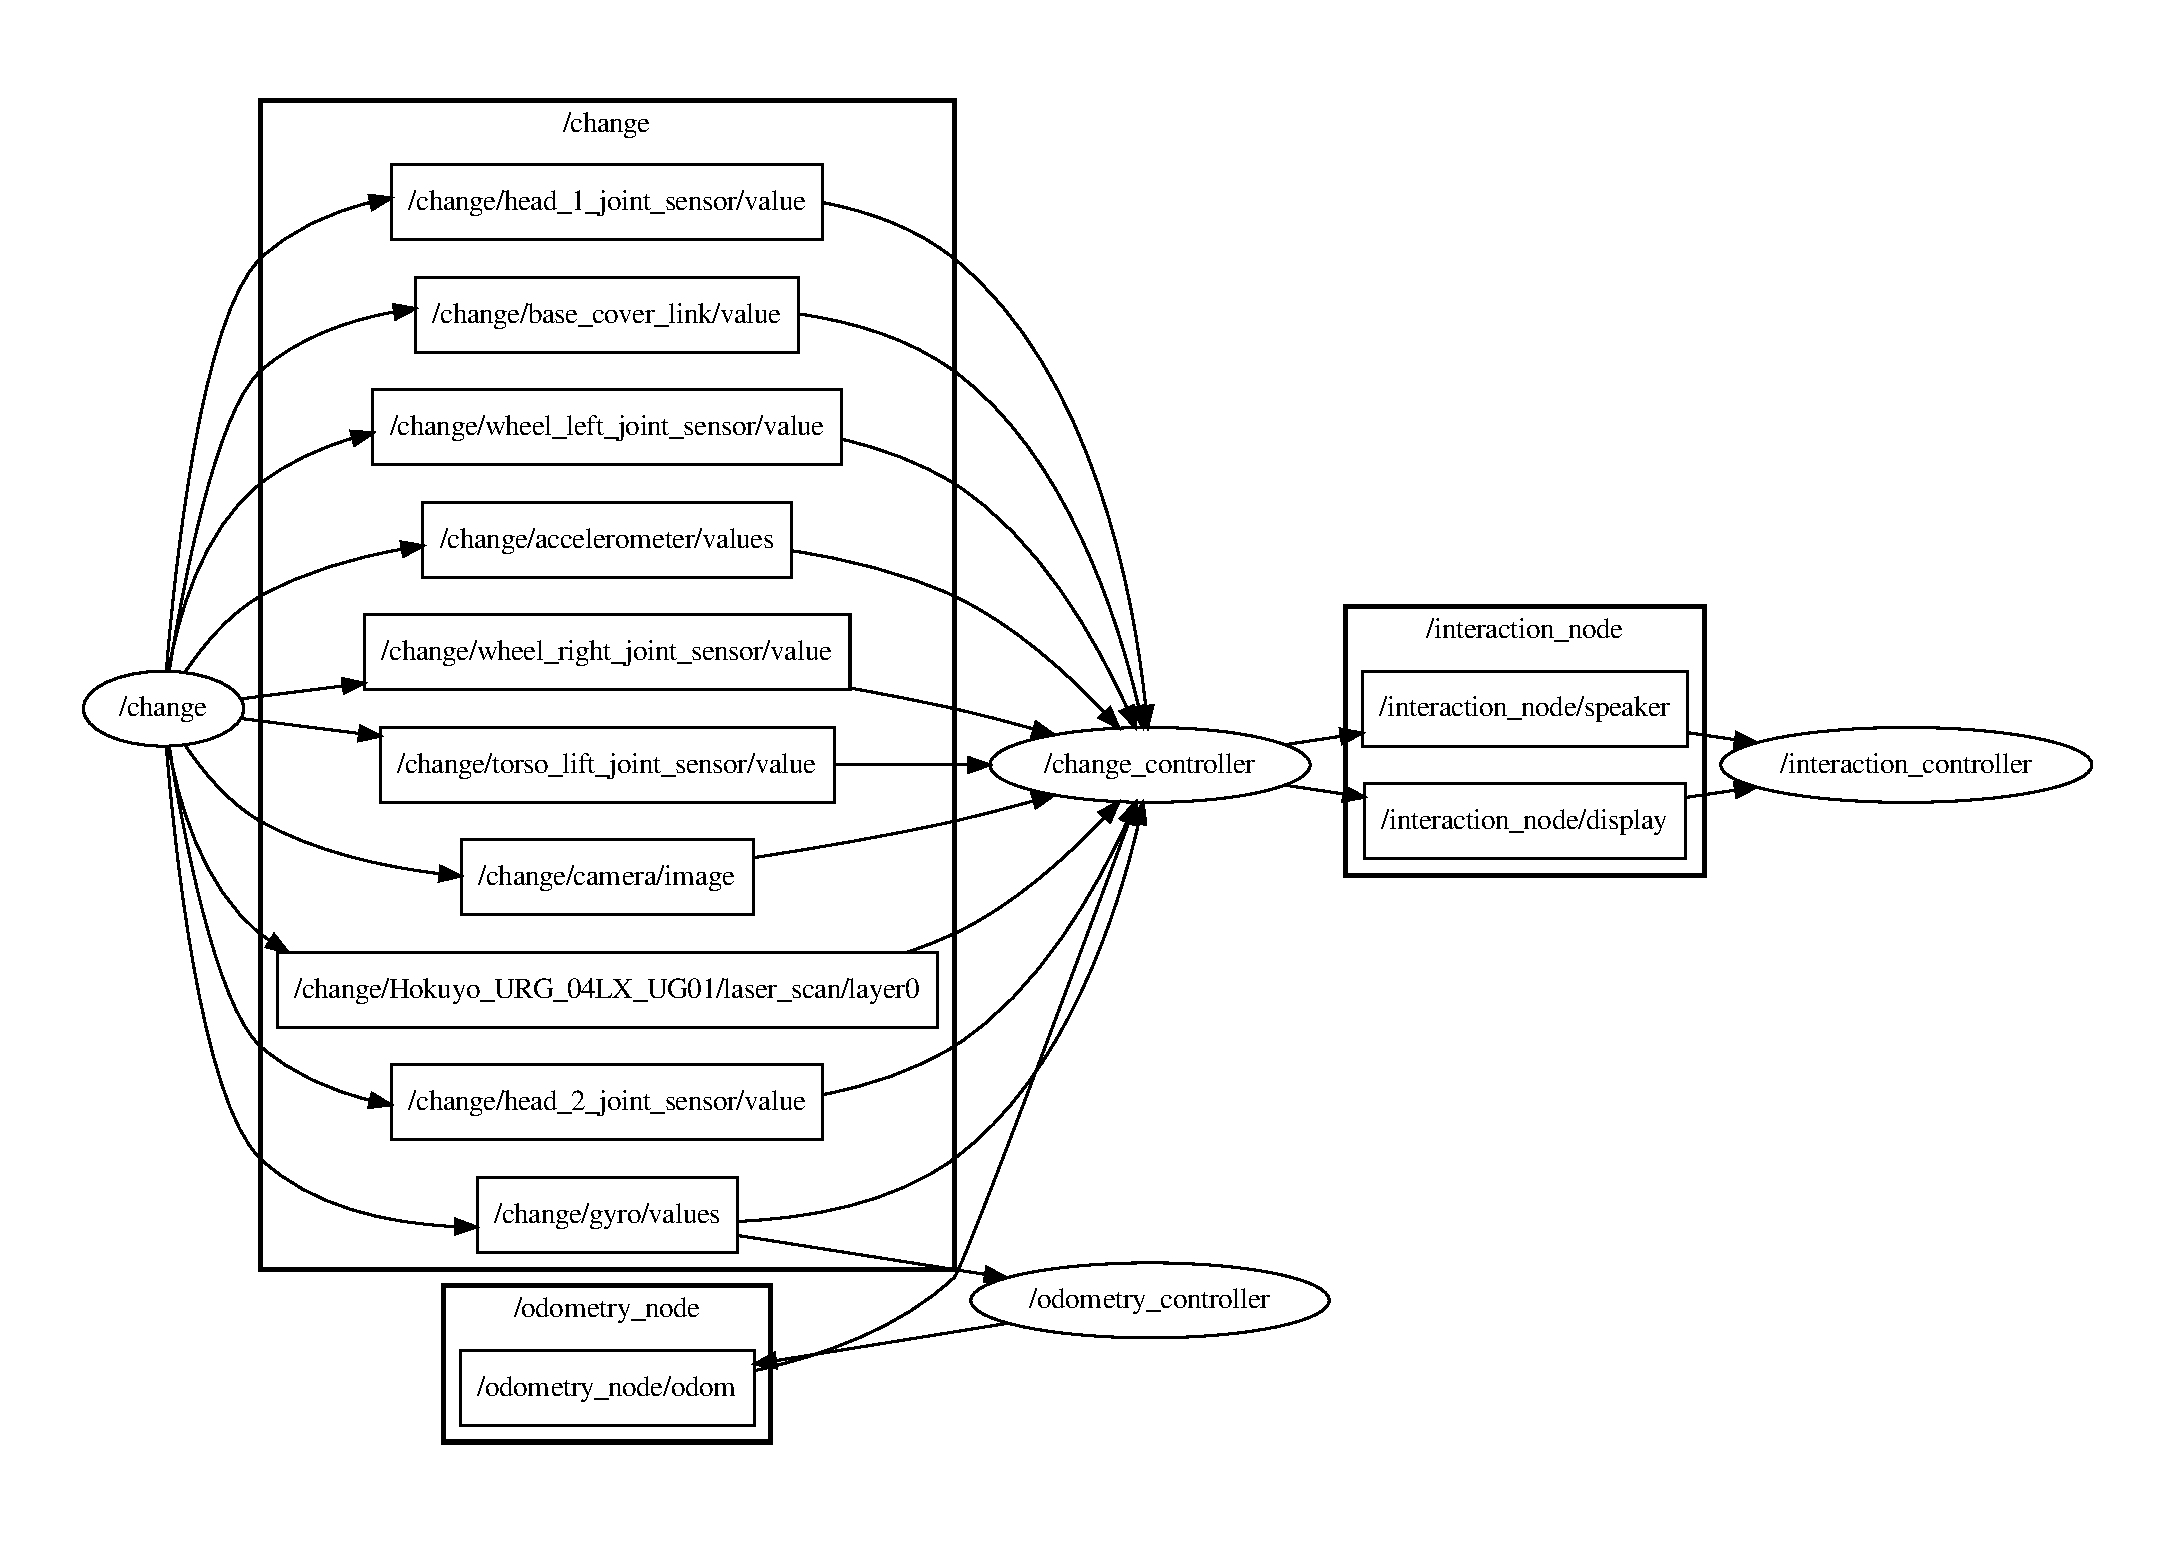
\includegraphics[width=1\textwidth]{img/rosgraph.pdf}
		\caption{Architettura dei nodi ROS, ottenuta tramite \textit{rqt}}
		\label{fig:rosgraph}
	\end{figure}
	}

	\begin{frame}{Webots node}
	Questo nodo si occupa solamente di lanciare Webots, e di impostare il
	valore del clock di ROS in base al tempo della simulazione, in modo da
	potere effettuare le integrazioni del tempo correttamente.
	\end{frame}
	\begin{frame}{Change controller node}
	Questo è il nodo che si occupa della gran parte della elaborazione. Oltre
	ad arbitrare sui comportamenti da assumere, gestisce più moduli che si
	occupano di: 
	\begin{itemize}
		\pause\item acquisire i dati dai sensori
		\pause\item mandare i comandi ai motori
		\pause\item gestire il movimento, quindi rotazioni e traslazioni
		\pause\item acquisire e analizzare le immagini dalla camera
	\end{itemize}
	\end{frame}

	\begin{frame}{Interaction node}
	Questo nodo ha il compito di gestire le interazioni audio/video. Ogni
	messaggio che viene riprodotto, prima in lingua italiana e poi inglese,
	viene anche visualizzato testualmente sullo schermo in italiano, inglese e
	cinese.  I possibili comportamenti assunti dal robot sono:
	\begin{itemize}
		\pause\item Salutare all'avvio
		\pause\item Mostrare sul display immagini che esortano a rispettare il
			distanziamento sociale
		\pause\item Riprodurre un messaggio audio che invita a rispettare il distanziamento sociale quando
			rileva un assembramento o quando scansiona l'ambiente
	\end{itemize}
	\end{frame}

	\begin{frame}{Odometry node}
	Il nodo che si occupa dell'odometria si occupa di stimare la posizione del
	robot, come spiegato approfonditamente nella
	sezione~\ref{sec:Modello-del-moto-e-posizionamento}. In generale ciò che fa
	è integrare costantemente i valori del giroscopio e della velocità delle
	ruote per condividere posizione e orientamento del robot.
	\end{frame}
	
	

	\section{Modello del moto e posizionamento}\label{sec:Modello-del-moto-e-posizionamento} 
	\frame{\sectionpage}
	
	\begin{frame}{Orientamento}
		Il modello del moto è caratterizzato da rotazioni e traslazioni. Per le
		rotazioni ci basiamo sui dati forniti dal giroscopio, il quale fornisce
		una velocità angolare. Calcoliamo quindi l'angolo di rotazione
		effettuando un'integrazione discreta dei campioni con interpolazione
		lineare del primo ordine (Eq.~\ref{eq:gyro-integration}).  
		\begin{equation}\label{eq:gyro-integration}
			\theta_i = \sum_{j=1}^i \frac{\omega _{j-1}+\omega _j}{2} \left( t_j-t_{j-1} \right) 
		\end{equation}
		Noto l'angolo corrente e l'angolo target utilizziamo un controllore
		proporzionale per raggiungere l'angolo desiderato.
	\end{frame}
	
	\begin{frame}{Spostamento}
		Per effettuare lo spostamento lineare utilizziamo il controllore PID
		
		(Proporzionale-Integrale-Derivativo) delle ruote fornito da Webots, che
		richiede un angolo di rotazione target per ogni ruota. Utilizziamo quindi
		l'angolo di rotazione corrente, e il diametro delle ruote per calcolare la
		posizione delle ruote necessaria al fine di ottenere lo spostamento
		desiderato (Eq.~\ref{eq:odometry}).
		\begin{equation}\label{eq:odometry}
		targetAngle =
		currentAngle+2\pi\frac    {distance}
						{2\pi \cdot diameter}
		\end{equation}
	\end{frame}
	
	\subsection{Posizionamento}\label{subsec:Posizionamento}
	\begin{frame}{Posizionamento}
		Inizialmente al segnale dell'accelerometro
		veniva applicato un integrale doppio per ottenere lo spostamento
		lineare(Eq.~\ref{eq:accel-integration} 	\cite{positioning}).
		
		\begin{equation}\label{eq:accel-integration}
			\begin{cases}
				\textbf{v}_i & = \sum_{j=1}^{i} \frac{\textbf{a} _{j-1}+\textbf{a} _j}{2} \left( t_j-t_{j-1} \right) \\
				\textbf{s}_i & = \sum_{j=1}^{i} \frac{\textbf{v} _{j-1}+\textbf{v} _j}{2} \left( t_j-t_{j-1} \right) 
			\end{cases}
		\end{equation}
		
		\pause
		Abbiamo ritenuto necessario cambiare approccio, decidendo di utilizzare
		gli encoders delle ruote per determinare gli spostamenti. 
		
		Integriamo la velocità lineare del robot, calcolata a partire dal
		raggio $R$ e le velocità angolari $u$ delle ruote.
		
		\begin{equation}\label{eq:linear-velocity}
			v_i = \frac{R (u_{r,i}+u_{l,i})}{2}
		\end{equation}
		
		\pause
		Questi valori sono aggiornati ad ogni intervallo di campionamento utilizzando la velocità lineare e la velocità angolare del robot \cite{572228}.
		
		\begin{equation}\label{eq:position-vector-update}
			\textbf{P}_i = \sum_{j = 1}^{i} \begin{bmatrix}
				 & v_j\cos(\theta_j ) & \\
				 & v_j\sin(\theta_j )
			\end{bmatrix}\cdot (t_j-t_{j-1}) 
		\end{equation}		
		
	\end{frame}
	\begin{frame}
		\begin{figure}[H]
			\begin{subfigure}{0.49\textwidth}
				\centering
				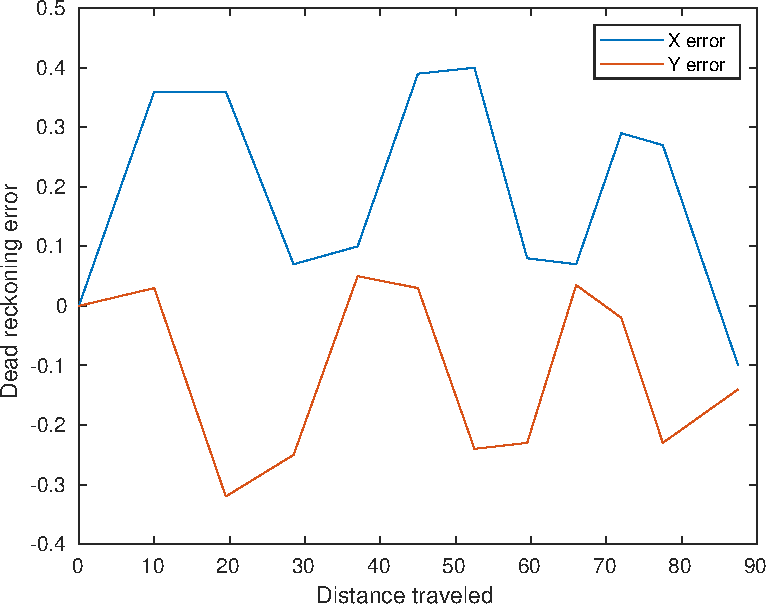
\includegraphics[width=0.8\linewidth]{./img/dead_reckoning_error.pdf}
				\caption{Errore nella stima della posizione}
				\label{fig:dead_reckoning_error}
			\end{subfigure}
			\begin{subfigure}{0.49\textwidth}
				\centering
				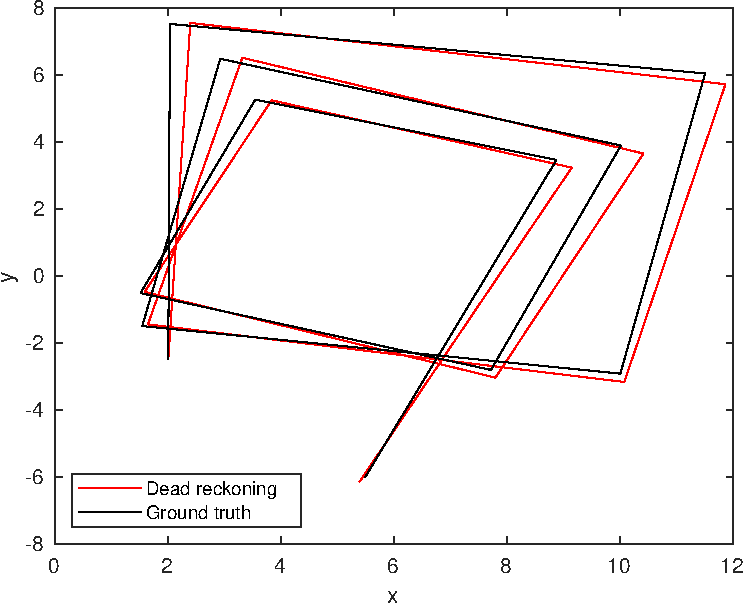
\includegraphics[width=0.8\linewidth]{./img/trajectories.pdf}
				\caption{Errore nella stima della traiettoria}
				\label{fig:trajectory_error}
			\end{subfigure}
		\end{figure}
		Abbiamo misurato le performance della stima di posizione e i risultati
		sono ritenuti soddisfacenti per raggiungere l'obbiettivo proposto.
	\end{frame}
	
	\begin{frame}{Collision avoidance}
		Il \textbf{TIAGo} è in grado di rilevare gli ostacoli grazie
		all'utilizzo di un sensore lidar.  
		
		Nell'immagine seguente viene mostrata la zona nella quale, se viene
		indicata dal lidar la presenza di un ostacolo, il \textbf{TIAGo} si
		ferma per ragioni di sicurezza al fine di evitare danni a persone e/o
		oggetti.
		\begin{figure}[H]
			\centering
			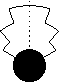
\includegraphics[width=0.2\textwidth]{./img/collision_avoidance.pdf}
			\caption{Collision avoidance}
			\label{fig:collision_avoidance}
		\end{figure}
	\end{frame}
	
	\section{Object recognition}\label{sec:Object-recognition}
	\frame{\sectionpage}
	
	\begin{frame}{Campionamento delle immagini}
		Il FOV della camera è di 57°, quindi per ricoprire 360° è necessario
		effettuare 7 campionamenti. Il settimo campionamento, come si vede in
		figura \ref{fig:campionamento_immagini}, è sovrapposto al primo per 39°.

		È possibile che un individuo si trovi in una zona di confine
		tra due campioni, e che quindi non sia correttamente identificabile in
		nessuna delle due immagini in cui appare parzialmente. Mitighiamo
		questo problema effettuiamo una rudimentale operazione di image
		mosaicing~\cite{ghosh2016survey} e campioniamo l'immagine così
		ottenuta ad intervalli di 28°.
		
		
		\begin{figure}[H]
			\centering
			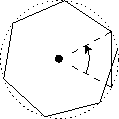
\includegraphics[width=0.3\textwidth]{./img/pictures_sampling.pdf}
			\caption{Campionamento delle immagini}
			\label{fig:campionamento_immagini}
		\end{figure}
	\end{frame}
	
	\begin{frame}{YOLO}
		Abbiamo valutato le performance di YOLOv3 (you only look once),\\
		YOLOv3-tiny, HoG, HoG + SVG. In seguito a vari test su HoG abbiamo
		ritenuto essere problematica la larghezza delle bounding boxes fornite.
		YOLOv3 fornisce risultati soddisfacenti.
		
		Considerando le caratteristiche hardware del robot mobile, abbiamo
		optato per l'uso di YOLOv3-tiny, il quale risulta essere
		significativamente più efficiente (approssimativamente del 442\%
		\cite{tiny_yolo}). Inoltre è rilevante in tal senso un paragone fra
		YOLOv3 e YOLOv3-tiny in termini di mAP (mean average precision) e FLOPS
		(floating-point operations per second) addestrate sul dataset COCO,
		come illustrato dalla tabella.
		
		\begin{table}[htpb]
			\centering
			\begin{tabular}{ c c c c } 
				\hline
				\textbf{Model} & \textbf{mAP} & \textbf{FLOPS} & \textbf{FPS} \\
				\hline	
				 YOLOv3-320    & 51.5  &  38.97  Bn  &  45  \\ 
				 YOLOv3-416    & 55.3  &  65.86  Bn  &  35  \\ 
				 YOLOv3-608    & 57.9  &  140.69 Bn  &  20  \\ 
				 YOLOv3-tiny   & 33.1  &  5.56   Bn  &  220 \\
				 YOLOv3-spp    & 60.6  &  141.45 Bn  &  20  \\
				\hline
			\end{tabular}
			\label{tab:comparison}
		\end{table}
	\end{frame}

	\section{Posizione dei target}\label{sec:Posizione-dei-target}
	\frame{\sectionpage}
	
	\subsection{Triangolazione}\label{subsec:Triangolazione}
	\begin{frame}{Triangolazione}
		\begin{columns}
			\begin{column}{0.4\textwidth}
				\begin{figure}[htpb]
					\centering
					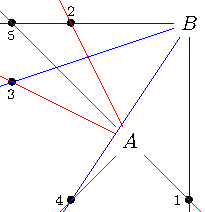
\includegraphics[width=\textwidth]{./img/ideal_object_triangulation.pdf}
					\label{fig:triangulation}
				\end{figure}
			\end{column}

			\begin{column}{0.6\textwidth}
				\justifying
				La triangolazione come metodo di individuazione delle persone
				presenta dei problemi nel nostro scenario:
				\begin{itemize}
					\justifying
					\pause\item Occlusione delle persone: se due persone
						(5 e 2) sono una dietro l'altra lungo una retta
						immaginaria che le congiunge al robot (B), quest'ultimo
						non sarà in grado di individuare la più distante. 

					\pause\item Imputazione delle osservazioni: quando il robot
						effettua scan successivi non è in grado di dedurre
						quali osservazioni derivano dalla stessa persona.
						Non è possibile determinare quali intersezioni
						corrispondono ad osservazioni reali e quali sono spurie. 

				\end{itemize}
			\end{column}
		\end{columns}
	\end{frame}
	
	\subsection{Calcolo della distanza}\label{subsec:Calcolo-della-distanza}
	\begin{frame}[allowframebreaks]{Calcolo della distanza}
		Ipotizzando che la camera abbia un FOV (field of view) di
		$2\alpha$ e sia distante $d$ dall'oggetto, la massima distanza
		orizzontale che un punto dell'immagine potrebbe avere dal centro del
		piano dell'immagine sarebbe $a = d \tan \alpha$.
		
		\begin{figure}[H]
			\centering
			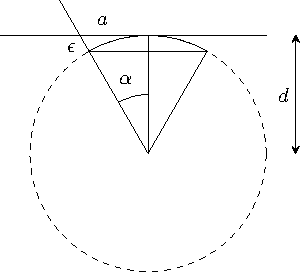
\includegraphics[width=0.4\textwidth]{./img/linearization_error.pdf}
		\end{figure}
		
		Ignorare la prospettiva significa effettuare un'approssimazione lineare
		del primo ordine e trattare il punto come se si trovasse su una
		circonferenza di raggio $d$ centrata sulla camera. Di conseguenza
		consideriamo il punto come se fosse più vicino di quanto non sia
		realmente, commettendo l'errore mostrato nell' Eq.~\ref{eq:max_err}.
		Con una camera con FOV di 1 radiante la sottostima è del 13.9\%.
		
		\begin{gather}
		\begin{aligned}
		\epsilon &= 
		\sqrt{a^2+d^2} - d =
		\sqrt{(d\tan \theta )^2+d^2}-d =\\
		&=d\left( \sqrt{\frac{1}{\cos ^2 \alpha}}-1 \right) =
		d \left( \sec \alpha -1 \right) 
		\end{aligned}
		\label{eq:max_err}
		\end{gather}
		
		\framebreak
		
		Poiché stiamo utilizzando un simulatore non è nota la larghezza del
		sensore da utilizzare per l'eq.~\ref{eq:obj_dist}. Abbiamo ovviato a
		tale problema posizionando il robot ed un oggetto dalle dimensioni note
		in posizioni note e abbiamo utilizzato questi dati insieme a delle
		misure in pixel nell' eq.~\ref{sensor_size}. Abbiamo così stimato le
		dimensioni del sensore virtuale da utilizzare nei calcoli successivi.
		
		\begin{equation}\label{eq:obj_dist}
		object~distance(m) = 
		\frac{f(m) \times real~width(m) \times image~width(pixels)}
		{object~width(pixels) \times sensor~width(m)}
		\end{equation}
		
		\begin{equation}\label{sensor_size}
		sensor~width(m) = 
		\frac{f(m) \times real~width(m) \times image~width(pixels)}
		{object~width(pixels) \times object~distance(m)}
		\end{equation}

	\end{frame}
	
	\subsection{Scarto dei duplicati}\label{subsec:Scarto-dei-duplicati}

	\begin{frame}[allowframebreaks]{Scarto dei duplicati}
		È stato necessario effettuare una fase di clustering al fine di
		scartare le bounding box duplicate. L'algoritmo di clustering
		utilizzato è DBSCAN (Density based scan) \cite{dbscan}, i cui parametri
		principali sono \textbf{eps}, ovvero la massima distanza fra due punti
		affinché vengano considerati appartenenti a un cluster ,
		\textbf{min\_samples}, ovvero il numero minimo di punti affinché un
		cluster sia valido (nel nostro caso è uguale a 1 in quanto non vogliamo
		scartare ROI) ed infine la metrica di distanza.
		
		\begin{figure}[H]
			\centering
			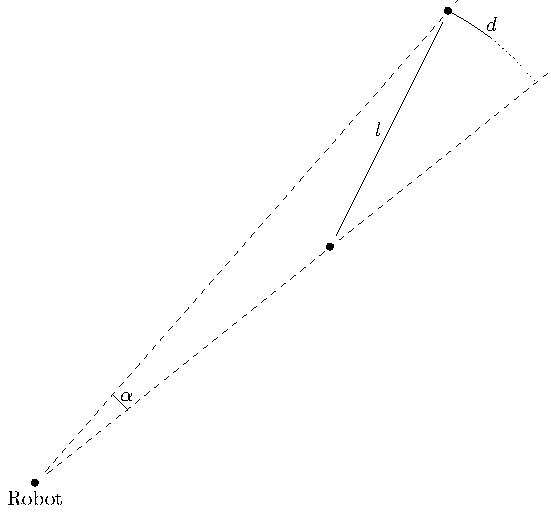
\includegraphics[width=0.4\textwidth]{./img/nms.pdf}
		\end{figure}
	\end{frame}

	\subsection{Correzione dei valori}\label{subsec:Correzione-dei-valori}
	\begin{frame}[allowframebreaks]{Correzione dei valori}
		Per migliorare la stima sulla distanza abbiamo paragonato le reali
		distanze dei target con le stime effettuate dal sistema ottenendo il
		polinomio interpolante $0.003116*x^5 - 0.09722*x^4 + 1.124*x^3
		-5.908*x^2 + 14.5*x-7.367$, che approssima la funzione di correzione della stima. 
		
		\begin{figure}[H]
			\centering
			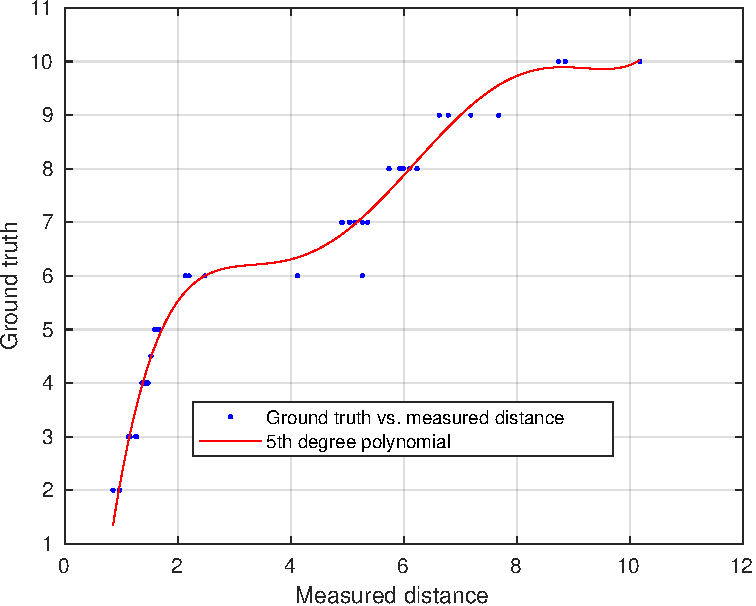
\includegraphics[width=0.6\textwidth]{./img/interpolation.pdf}
			\label{fig:interpolation}
		\end{figure}

	\framebreak
	
	Le bontà della stima della distanza e dell'angolo si evince dalle figure :

	\begin{figure}[ht]
		\begin{subfigure}{.49\textwidth}
			\centering
			% include first image
			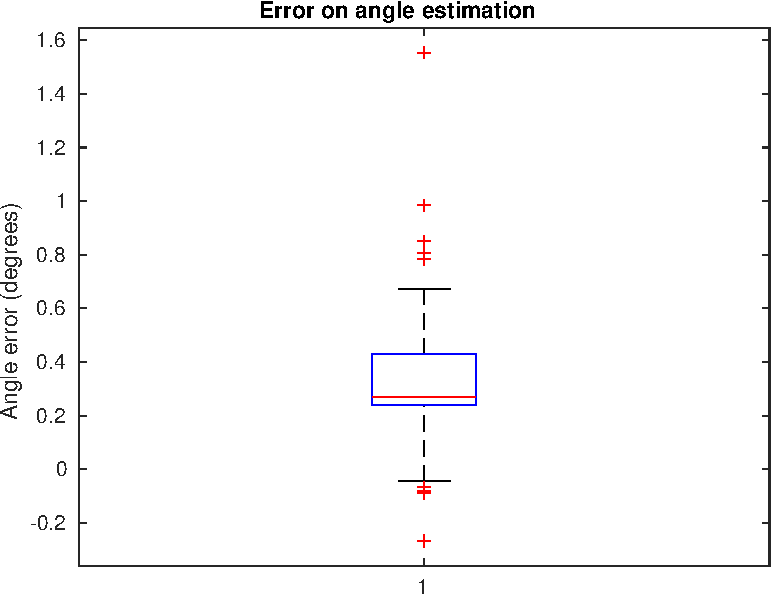
\includegraphics[width=1\linewidth]{./img/angle_error.pdf}  
			\label{fig:angle_plot}
		\end{subfigure}
		\begin{subfigure}{.49\textwidth}
			\centering
			% include second image
			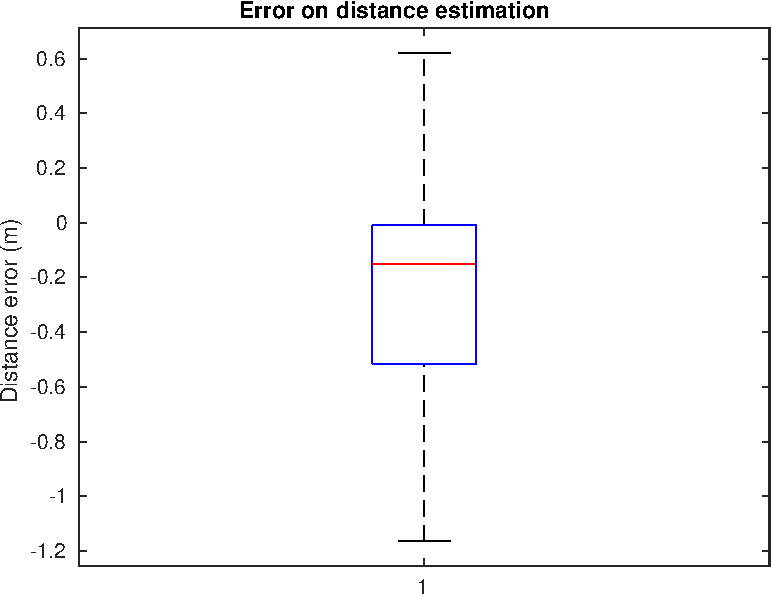
\includegraphics[width=1\linewidth]{./img/distance_error.pdf}  
			\label{fig:distance_plot}
		\end{subfigure}
		\caption{Box plot relativi all'errore su angolo e distanza}
		\label{fig:boxes_plot}
	\end{figure}

	\framebreak

	Nelle figure viene riportata la distribuzione gaussiana multivariata
	in 3 e 2 dimensioni con matrice di covarianza calcolata dai nostri test :
	\begin{figure}[H]
		\begin{subfigure}{0.49\linewidth}
			\centering
			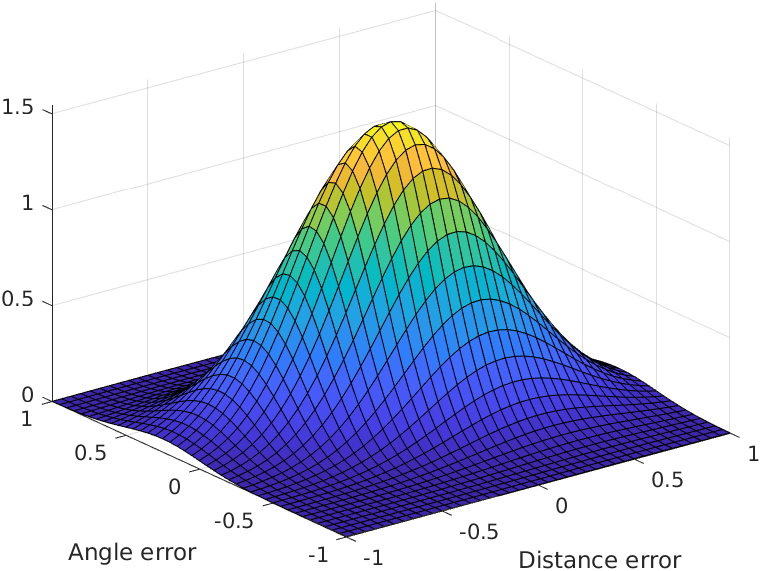
\includegraphics[width=\textwidth]{./img/error_covariance.png}
			\label{fig:error_covariance}
		\end{subfigure}
		\begin{subfigure}{0.49\linewidth}
			\centering
			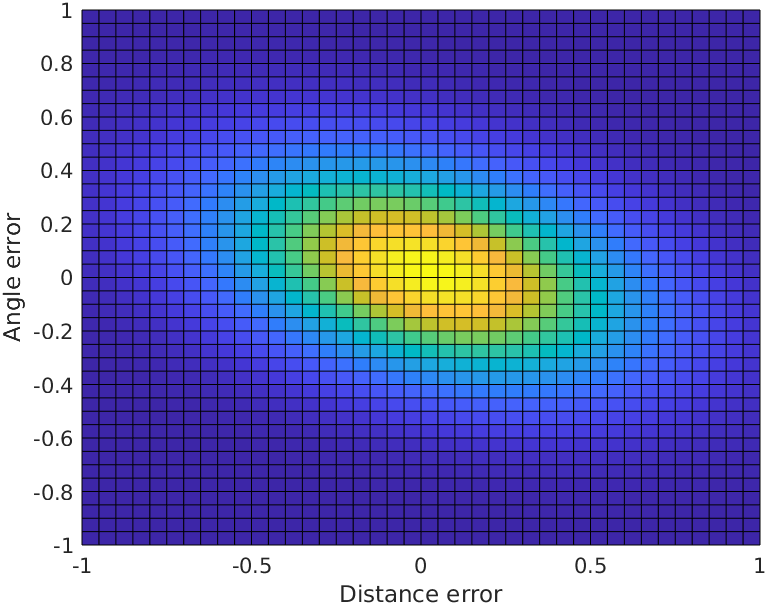
\includegraphics[width=\textwidth]{./img/error_covariance_flat.png}
			\label{fig:error_covariance_flat}
		\end{subfigure}
	\end{figure}

	\end{frame}

	\section{Modello probabilistico}\label{sec:Modello-probabilistico}
	\frame{\sectionpage}
	\begin{frame}{Modello probabilistico}
	Nella nostra applicazione la distanza stimata
	dell'oggetto sarà soggetta ad errore non trascurabile. Per questa
	ragione e per i problemi legati alla triangolazione abbiamo abbandonato la
	rappresentazione basata su oggetti e abbiamo fatto ricorso ad un filtro di
	occupazione bayesiano (BOF)~\cite{tay2008bayesian}.
	
	Nel filtro di occupazione bayesiano, il problema dell'associazione dei dati viene superato in quanto
	viene gestito da un livello di astrazione superiore. Il concetto di oggetto
	viene difatti riformulato da proprietà più utili quali occupazione o
	rischio, che vengono stimate direttamente per ogni cella utilizzando sia
	osservazioni dai sensori che conoscenze pregresse. Le caratteristiche di
	incertezza legate ai sensori vengono descritte, in questo modello,
	attraverso le probabilità di occupazione.
	\end{frame}
	\begin{frame}{Funzione densità di probabilità I}
	
	Al fine di trasformare le osservazioni ottenute in una probabilità che le
	persone si trovino effettivamente nella posizione indicata è stato
	necessario definire una funzione densità di probabilità. La distribuzione
	normale è computazionalmente onerosa. Abbiamo quindi fatto ricorso ad una approssimazione (Eq.~\ref{eq:pdf}).
	
	
	
	\begin{figure}[ht]
		\centering
		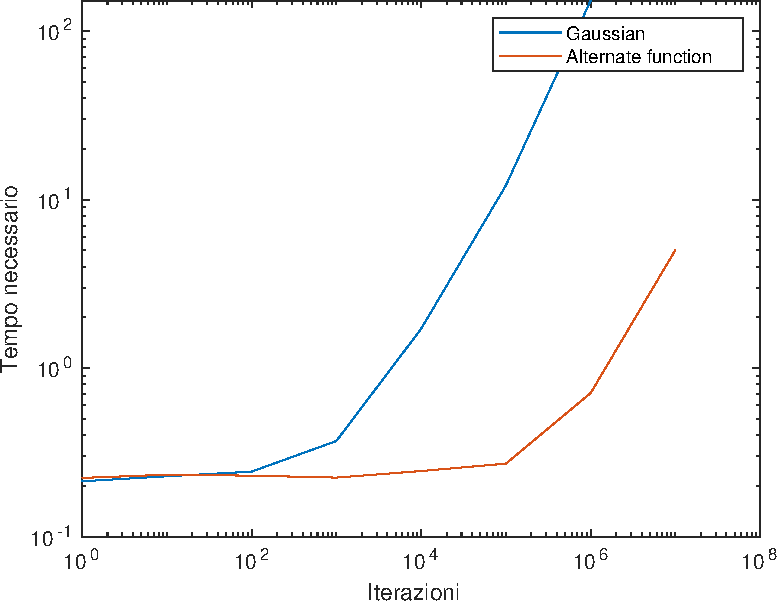
\includegraphics[width=0.6\linewidth]{./img/pdf_benchmark.pdf}
		\label{fig:pdf_benchmark}
	\end{figure}
	
	\end{frame}
	\begin{frame}{Funzione densità di probabilità II}
	
	La distribuzione triangolare è spesso utilizzata per approssimare una
	gaussiana, tuttavia, presenta delle caratteristiche non volute per il
	nostro caso d'uso. 
	
	\begin{itemize}
		\pause\item Non presenta le "fat tails"
		\pause\item Dopo una prima osservazione non confermata successivamente la probabilità scende a zero.
		\pause\item Le occlusioni annullano la probabilità
		\pause\item I target in movimento non verrebbero rilevati
	\end{itemize}
	
	\pause Essendo la scansione una operazione estremamente costosa non è nemmeno
	possibile affidarsi esclusivamente all'aggiunta di rumore alla griglia di
	occupazione confidando in una eventuale convergenza.

	\end{frame}
	\begin{frame}{Funzione densità di probabilità III}

	Al fine di ottenere un'approssimazione di una gaussiana adatta al
	nostro scenario, per modellare la probabilità che data l'occupazione della
	cella in posizione $ {\bf x} $ si ottenga l'osservazione $ {\bf z} $, è
	stato utilizzato un funzionale ispirato al guadagno del filtro di
	Butterworth.

	\begin{equation}\label{eq:pdf}
	p({\bf z}|{\bf x}) = \frac	{K}
	{1 + d({\bf x},{\bf z})^4 } 
	\end{equation}
	
	\begin{figure}[ht]
		\centering
		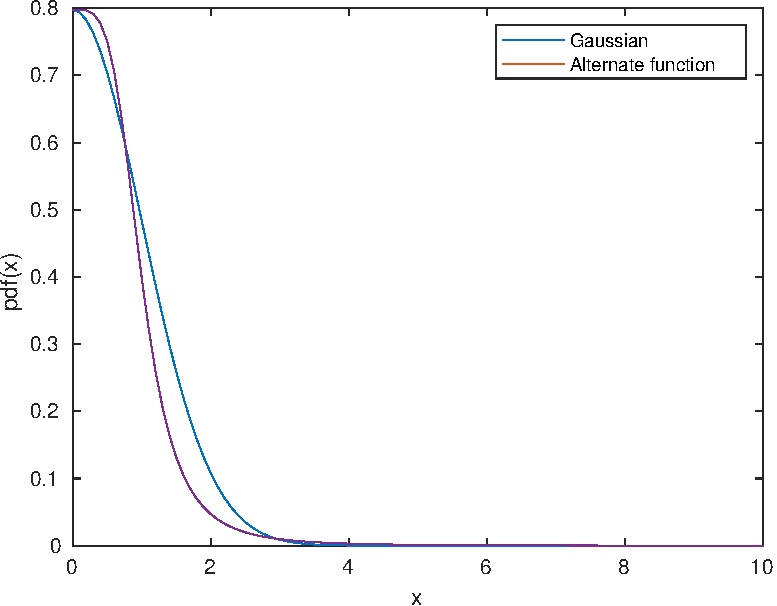
\includegraphics[width=0.5\linewidth]{./img/pdf_shape.pdf}
		\label{fig:pdf_shape}
	\end{figure}
	
	
	\end{frame}
	\begin{frame}[allowframebreaks]{Parametri PDF}
	
	La distanza euclidea nell'equazione~\ref{eq:pdf} porterebbe a formare aree ad alta probabilità di forma
	circolare. Questo però non si adatterebbe bene al nostro modello di errore
	del sensore: l'angolo dell'oggetto rispetto al robot è noto con una
	precisione molto elevata, mentre la maggior parte dell'incertezza si
	concentra nella distanza. Calcoliamo quindi la distanza non come distanza
	euclidea tra le coordinate cartesiane della cella e dell'osservazione, ma
	come norma $L^2$ delle coordinate polari, opportunamente normalizzate per
	tenere conto della diversa incertezza sulla misura di angolo e distanza.
	
	\framebreak

	L'incertezza sulla distanza è ricavata dalle misure di calibrazione
	effettuate. Per l'angolo è stato seguito un approccio differente:
	utilizzare una varianza calcolata a partire da una serie di osservazioni
	porterebbe ad assegnare maggiore probabilità ad oggetti lontani. \\
	In un
	setup come quello in figura~\ref{fig:circular_sector}, con due target
	rilevati, rispettivamente a distanza $d_1$ e $d_2$, le aree ad alta
	probabilità relative ad entrambi i punti avranno lunghezza $l$ e ampiezze $
	\alpha_1 \text{ e } \alpha_2  $. 
	
	\begin{figure}[H]
		\centering
		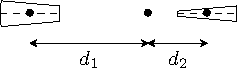
\includegraphics[width=0.5\textwidth]{img/circular_sector.pdf}
		\caption{Area della regione probabile a seconda della distanza.}
		\label{fig:circular_sector}
	\end{figure}

	La dimensione dell'area ad alta probabilità è direttamente
	proporzionale alla distanza e all'ampiezza dell'angolo. Se quindi $
	\alpha_1 $ coincidesse con $ \alpha _2 $ ad oggetti distanti verrebbero
	associate aree molto più grandi. 
	\begin{subequations}\label{eq:circular_sector}
	\begin{align*} 
		A_1  = & \pi((d_1+l/2)^2-(d_1-l/2)^2)\frac{\alpha_1}{2\pi}  =  \alpha_1 d_1l \\
		A_2  = & \pi((d_2+l/2)^2-(d_2-l/2)^2)\frac{\alpha_2}{2\pi}  =  \alpha_2 d_2l \\
\tag{\ref{eq:circular_sector}}
		\frac{A_1}{A_2} = & \frac	{\alpha_1 d_1} {\alpha_2 d_2}
	\end{align*}
	\end{subequations}
	
		
	Per evitare questo problema, dopo avere
	individuato un valore $ \alpha ^* $ appropriato questo viene scalato per un
	coefficiente inversamente proporzionale alla distanza della cella, quindi $
	\alpha _1 = \alpha ^*/d_1 $ e $ \alpha _2=\alpha ^*/d_2 $, da cui $A_1=A_2$. 
	
	\end{frame}
	\begin{frame}{Aggiornamento bayesiano I}
	
	Dato un insieme di osservazioni ottenute da una scansione $ Z_i $ aggiorniamo il belief.
	\begin{equation}\label{eq:belief-update}
		p({\bf x}_i | Z_i) = p({\bf x}_{i-1}) \cdot 
		\sum_{{\bf z} \in Z_i} p({\bf z} | {\bf x}_i)
	\end{equation}

	Questa formula è valida sotto le seguenti assunzioni:
	\begin{itemize}
		\pause\item In uno stesso scan, date due osservazioni $z_1$ e
			$z_2$ queste non hanno intersezione, quindi $ p(z_1 \cup z_2) =
			p(z_1)+p(z_2)-p( z_1 \cap z_2) = p(z_1)+p(z_2) $ 

		\pause\item In assenza di nuove osservazioni la stima dello stato del sistema
			rimane invariata: $ \overline{bel}(x_i) = bel(x_{i-1}) $ 

	\end{itemize}
	
	\end{frame}
	\begin{frame}{Aggiornamento bayesiano II}

	In mancanza di nuovi dati si potrebbero tentare due approcci:
	resettare le stime o lasciarle del tutto invariate. 
	\begin{itemize} 
		\pause\item Lasciare invariato il belief a seguito di multiple scansioni
			senza successo porterebbe a non notare che tutte le persone
			nell'ambiente in cui ci si trova sono andate via, continuando a
			considerare valide tutte le posizioni precedenti.
		\pause\item Dall'altro lato, un approccio troppo drastico quale
			immediatamente scartare tutte le precedenti stime porterebbe a
			perdere informazioni utili a causa di occlusioni temporanee
	\end{itemize}
	
	\pause Effettuiamo uno smoothing degli istogrammi
	prima di ogni update e aggiungiamo inoltre del rumore. 
	
	\end{frame}
	\begin{frame}{Individuazione dei cluster}
	
	Al fine di individuare le zone con alta probabilità di contenere persone, 
	in primo luogo effettuiamo una sogliatura utilizzando il metodo Otsu~\cite{otsu}, 
	ottenendo così una mappa binaria.
		
	Estraiamo le regioni ad alta probabilità contigue
	ed i loro contorni~\cite{contours} e selezioniamo come centro il punto
	con maggiore probabilità.

	\begin{figure}[H]
		\centering
		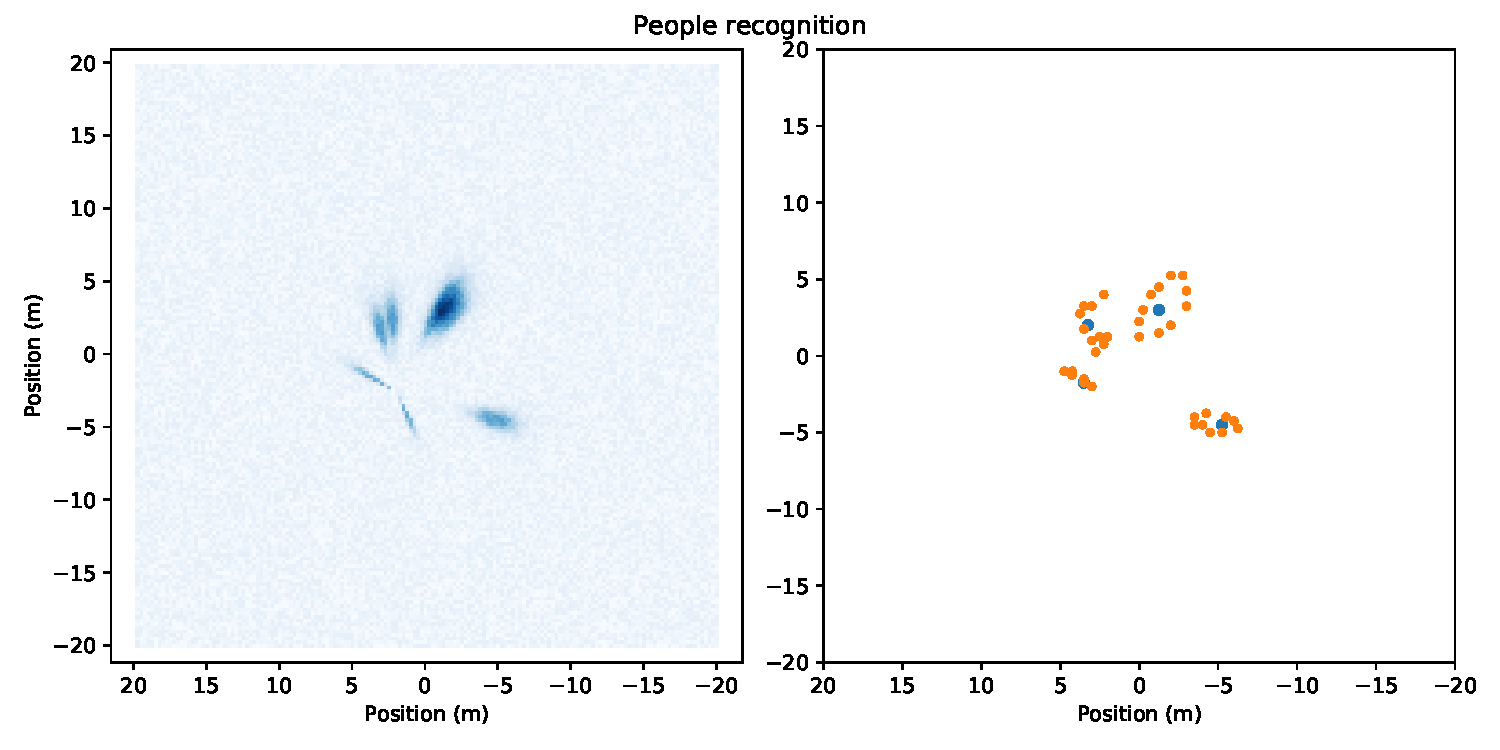
\includegraphics[width=0.8\textwidth]{./img/image_segmentation.pdf}
	\end{figure}

	\end{frame}
	
	\section{Scheduling dei comportamenti}\label{sec:Scheduling-dei-comportamenti}
	\frame{\sectionpage}
	\subsection{Modalità esplorazione}\label{subsec:Modalita-esplorazione}
	\begin{frame}{Modalità esplorazione}
	Quando il robot entra in modalità esplorazione il suo comportamento è di
	esplorazione casuale della mappa. Il robot continua ad esplorare ed
	effettuare scan periodici fino a quando non viene rilevato un obbiettivo.
	In tal caso il robot entra in modalità campi di potenziale. Se il robot
	incontra un ostacolo nel suo cammino ruota di $90^{\circ}$ nella direzione
	con più spazio e continua l'esplorazione casuale.
	\end{frame}
	
	\subsection{Bug mode}\label{subsec:Bug-mode}
	\begin{frame}{Bug mode}
	Quando il robot entra in modalità bug~\cite{503814} effettuiamo uno scan lidar. 
	Confrontiamo i valori ottenuti con una
	soglia al fine di individuare le discontinuità nel profilo degli ostacoli. 
	Analizziamo successivamente le discontinuità del segnale,
	corrispondenti ai bordi degli ostacoli.
	Da tali punti viene calcolato l'angolo fra la retta che li
	congiunge con l'obbiettivo. Il robot si muove infine verso il punto al
	quale corrisponde l'angolo minore, che ci farà allontanare meno
	dall'obbiettivo.
	
	\begin{figure}[H]
		\centering
		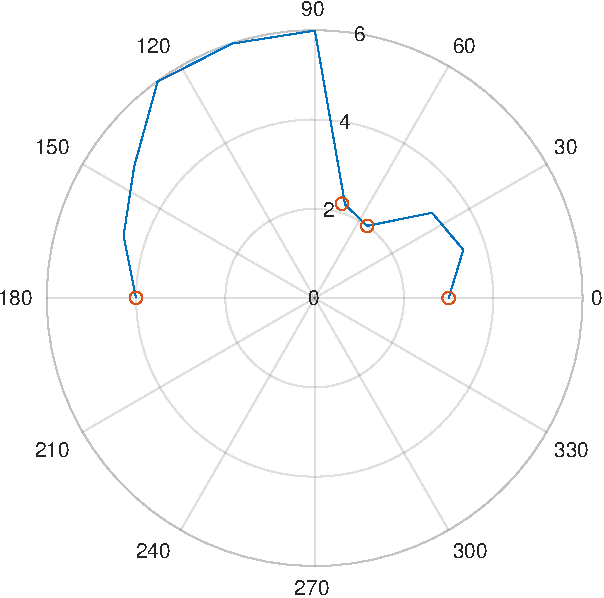
\includegraphics[width=0.4\textwidth]{./img/bug.pdf}
		\label{fig:bug}
	\end{figure}

	\end{frame}
	\subsection{Campi di potenziale}\label{subsec:Campi-di-potenziale}
	\begin{frame}{Campi di potenziale}
	\only<1>{
		\framesubtitle{Potenziale attrattivo}
		
		I modelli basati sui campi di potenziale richiedono la definizione di 
		potenziali attrattivi e repulsivi.
			
		Il potenziale attrattivo è centrato sul target, ed è modellato come un
		potenziale quadratico, la forza attrattiva è quindi lineare rispetto alla
		distanza (Eq.~\ref{eq:attractive-force}).

		\begin{equation}\label{eq:attractive-force}
			F_{att}( \textbf{x}) = k_a\cdot \left| {\bf x - x_d} \right| 
		\end{equation}
	}
   \stepcounter{equation}

	\only<2>{
		\framesubtitle{Potenziale repulsivo}
		Gli ostacoli generano invece un potenziale repulsivo. Questo ha un
		raggio d'azione limitato, la forza repulsiva è massima per un ostacolo
		a distanza nulla, e decresce in modo monotono fino ad annullarsi se la
		distanza dell'ostacolo supera una soglia $d_t$ con la legge descritta
		nell'equazione:

		\begin{equation}\label<2>{eq:repulsive-force}
			F_{rep}(distance) = \begin{cases}
				k_r \cdot \left(
					\frac{1}{distance^2}-
					\frac{1}{d_t^2}
				\right)  & distance \leq d_{t} \\
				0 & d > d_{thresh}
			\end{cases}
		\end{equation}
	}
	
	\begin{figure}[H]
		\centering
		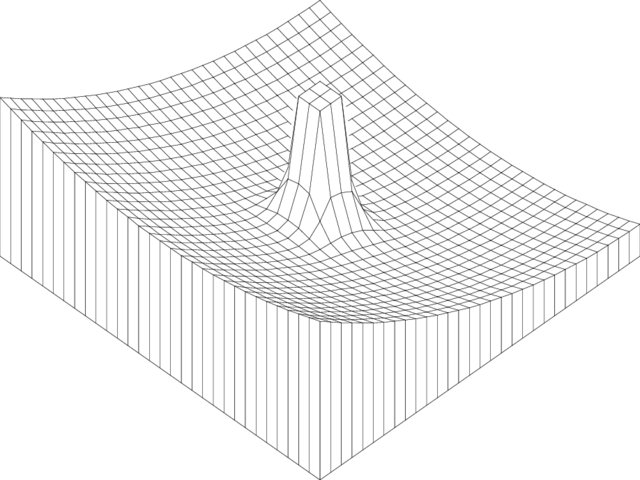
\includegraphics[width=0.4\textwidth]{./img/potential_field.jpg}
		\label{fig:potential_field}
	\end{figure}
	\end{frame}

	\begin{frame}{Campi di potenziale}{Rilevamento dell'ostacolo}

	La maggior parte dei potenziali repulsivi descritti in letteratura
	dipendono esclusivamente dalla distanza dall'ostacolo, interferendo con il
	moto anche se questo avviene parallelamente all'ostacolo. Per ovviare a
	questo problema prendiamo in considerazione solo gli ostacoli situati in un
	FOV frontale al robot con ampiezza $ \alpha  $ calcolata per permettere di
	muoversi parallelamente ad una superficie mantenendo una distanza di
	sicurezza $ h $ : 

	\begin{equation}\label{eq:obstacle_fov}
		\alpha = {2}\sin^{-1}{\frac{h}{d_t}}
	\end{equation}

	\begin{figure}[H]
		\centering
		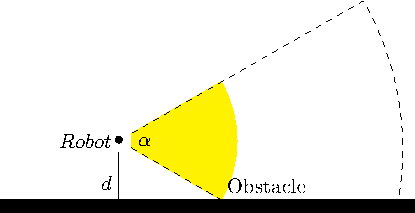
\includegraphics[width=0.5\textwidth]{./img/obstacle_fov.pdf}
		\caption{FOV frontale del robot}
		\label{fig:obstacle_fov}
	\end{figure}
	
	\end{frame}
	\begin{frame}{Campi di potenziale}{Calcolo del movimento}

	L'approccio seguito consiste in due comportamenti calcolati
	indipendentemente: il comportamento traslatorio e il comportamento
	rotazionale.

	La traslazione viene calcolata in funzione dello spazio di movimento a
	disposizione e dall'angolo rispetto al target secondo
	l'equazione~\ref{eq:translation}, ottenuta per interpolazione del profilo
	desiderato. L'angolo viene invece determinato dalla somma vettoriale delle
	forze attrattive e repulsive. La rotazione viene inoltre sogliata per
	evitare cambi di direzione troppo bruschi(Eq.~\ref{eq:angle}).

	\begin{equation}\label{eq:translation}
		d = 0.5 + \frac	{0.9\cdot distance - 0.5}
		{1 + \left|
				\frac{6\omega}{\pi}
		\right|  } 
	\end{equation}
	
	\begin{equation}\label{eq:angle}
		\omega = \begin{cases}
			\omega^*=\theta - \angle\left( \textbf{F}_{att} - \textbf{F}_{rep} \right)  & -\Omega \le \omega^* \le \Omega \\
			-\Omega & \omega^* < -\Omega \\
			\Omega & \omega^* < \Omega

		\end{cases}	\end{equation}
	
	\subsection{Automa a stati finiti}\label{subsec:Pianificazione}
	
	\end{frame}
	\begin{frame}{Automa a stati finiti}
	\begin{columns}
		\begin{column}{0.3\textwidth}
			\begin{figure}[H]
				\hfuzz=42pt 
				\centering
				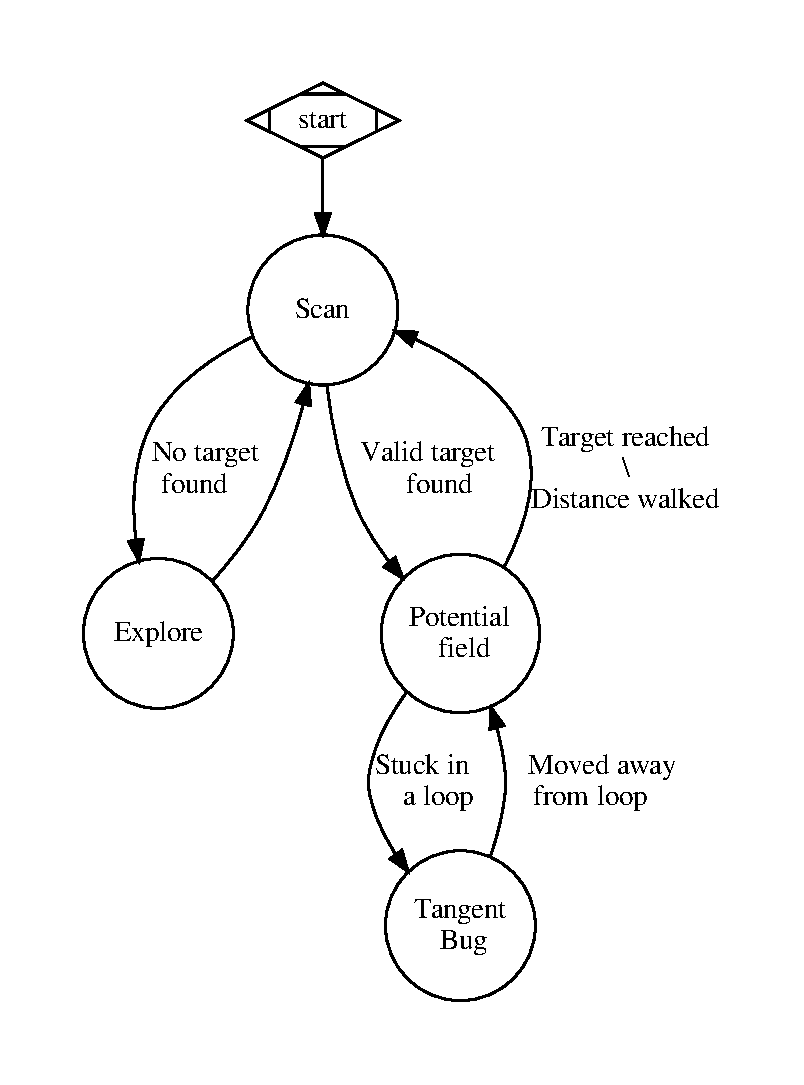
\includegraphics[width=1.45\textwidth]{./img/fsa.pdf}
				\label{fig:fsa}
			\end{figure}
		\end{column}	
		\begin{column}{0.7\textwidth}
		\justifying
		\begin{itemize}[<+->]
			\item All'avvio, \textbf{Change} effettua uno scan dell'ambiente.
			\item Se non vengono rilevati obbiettivi entra in modalità
				esplorazione e, dopo aver percorso una determinata distanza,
				effettua un nuovo scan
			\item Se viene rilevato un obbiettivo il robot entra in modalità
				campi di potenziale fermandosi una volta raggiunto l'obbiettivo
				o percorso una determinata distanza.
			\item Se, in modalità campi di potenziale, il \textbf{TIAGo} rimane
				bloccato in un loop, entra in modalità bug fino all'uscita dal loop, e ritorna nella modalità campi di
				potenziale.
		\end{itemize}
		\end{column}
	\end{columns}	
	\end{frame}
	
	\section{Possibili modifiche}\label{sec:Possibli-modifiche}
	\frame{\sectionpage}
	\frame{
	Riportiamo di seguito possibili modifiche da apportare:
		\begin{itemize}[<+->]
			\item Aggiungere un algoritmo per effettuare SLAM, in modo da poter
				pianificare il moto con algoritmi come A* \cite{A*} o RRT
				\cite{RRT}
			\item Migliorare la modalità Tangent Bug
			\item Utilizzare una depth-cam per stimare con più precisione la
				distanza delle persone
			\item Tracciamento delle persone in real-time
		\end{itemize}
	}

	\section{Conclusioni}\label{sec:Conclusioni}
	\frame{\sectionpage}
	\frame{
		Durante lo sviluppo del progetto sono state affrontate numerose
		tematiche trattate durante il corso di \textit{Robotica}. L'esperienza
		di sviluppo ha permesso al team di apprezzare l'importanza di solide
		fondamenta teoriche unite ad una significativa esperienza pratica. In
		particolar luogo abbiamo riscontrato problemi concernenti vari ambiti,
		dalla robotica probabilistica all'esplorazione degli ambienti, la cui
		ricerca di risoluzione ci ha portato ad approfondire le fondamenta
		teoriche della materia. La performance raggiunta, nonostante le
		tempistiche, risulta soddisfacente.
	}


	\subsection{Bibliografia}\label{subsec:Bibliografia}
	\begin{frame}[allowframebreaks]{Bibliografia}
		% Bibliography
		\bibliographystyle{unsrt}
		\bibliography{references.bib}
	\end{frame}

\end{document}
